\documentclass[10pt]{beamer}

%% Based on the original theme by Matthias Vogelgesang
%% 		https://github.com/hsrmbeamertheme/hsrmbeamertheme
%% Also Based on the UNC Charlotte theme by Benjamin Radford
%% 		https://github.com/matze/mtheme
%% This theme is licensed under a Creative Commons Atribution-ShareAlike 4.0 international license
%% For more info, see http://creativecommons.org/licenses/by-sa/4.0/
%%
%% Source obtained from:
%% https://www.overleaf.com/latex/templates/unc-charlotte-beamer-theme/rnwqwjmrnmsk

\usetheme[progressbar=frametitle]{metropolis}
\usepackage{appendixnumberbeamer}
\usepackage{booktabs}
\usepackage[scale=2]{ccicons}
\usepackage{pgfplots}
\usepgfplotslibrary{dateplot}

\usepackage{xspace}
\newcommand{\themename}{\textbf{\textsc{metropolis}}\xspace}

%%%%%%%%%%%%%%%%%%%%%%%%%%%%
%% Theme Adjustments %%
%%%%%%%%%%%%%%%%%%%%%%%%%%%%
\definecolor{CanvasBG}{HTML}{FAFAFA}

% Supporting Color Palette
\definecolor{White}{HTML}{FFFFFF}
\definecolor{WarmGray}{HTML}{696158}
\definecolor{StoneGray}{HTML}{717C7D}
\definecolor{DarkGreen}{HTML}{13381a}
\definecolor{LightGreen}{HTML}{509E2F}
\definecolor{BrightGold}{HTML}{F0CB00}
\definecolor{Royal}{HTML}{72246C}
\definecolor{Ocean}{HTML}{006BA6}
\definecolor{Flash}{HTML}{B52555}
\definecolor{Ruby}{HTML}{b50e0e}
\definecolor{Citrus}{HTML}{FFB81C}
\definecolor{Spring}{HTML}{CEDC00}
\definecolor{Garden}{HTML}{B7CE95}
\definecolor{Sand}{HTML}{F0E991}
\definecolor{Bloom}{HTML}{F1E6B2}
\definecolor{Clay}{HTML}{B7B09C}
\definecolor{Steel}{HTML}{b7b5ba}
\definecolor{Meteorite}{HTML}{404040}
\definecolor{Cloud}{HTML}{BAC5B9}


% Set colors here
\setbeamercolor{frametitle}{bg=Meteorite}
\setbeamercolor{progress bar}{bg=Steel, fg=Meteorite}
\setbeamercolor{alerted text}{fg=Ruby}

\setbeamercolor{block title}{bg=Meteorite, fg=White}
\setbeamercolor{block title example}{bg=Ocean, fg=White}
\setbeamercolor{block title alerted}{bg=Citrus, fg=White}
\setbeamercolor{block body}{bg=CanvasBG}

\metroset{titleformat=smallcaps, progressbar=foot}

\makeatletter
\setlength{\metropolis@progressinheadfoot@linewidth}{2pt}
\setlength{\metropolis@titleseparator@linewidth}{2pt}
\setlength{\metropolis@progressonsectionpage@linewidth}{2pt}
%%%%%%%%%%%%%%%%%%%%%%%%%%%%
%% Theme Adjustments %%
%%%%%%%%%%%%%%%%%%%%%%%%%%%%


\title{Real-Time Object Detection at the Edge}
\subtitle{Project Introduction and Goals}
\date{June 14, 2021}
\author{Colin Burdine}
\institute{SULI Intern, Hosted at Argonne National Laboratory}
% \titlegraphic{\hfill\includegraphics[height=1.5cm]{logo.pdf}}

\begin{document}

\maketitle

%\begin{frame}{Table of contents}
%  \setbeamertemplate{section in toc}[sections numbered]
%  \tableofcontents%[hideallsubsections]
%\end{frame}

\section{Introduction}

\begin{frame}{About Myself}
\begin{center}
\includegraphics[scale=0.25]{figures/me}
\end{center}
\begin{itemize}
\item I am a recent graduate of Baylor University (Sic 'Em Bears!)
\item I majored in Mathematics and Computer Science.
\item I am currently working on my Master's at Baylor, doing research in the field of quantum computing.
\end{itemize}
\end{frame}

\begin{frame}{Problem Statement}

\begin{itemize}
\item Over the past three to four decades, advances in computer vision systems and machine learning have enabled high-fidelity object detection, classification, and tracking.

\item However, these computer vision models and methods are often quite complex and perform poorly on small computing devices.

\pause 
\item This poses a challenge if we want to integrate these methods into an \alert{edge computing} system like Waggle:\\[4mm]
\begin{center}
\includegraphics[scale=0.4]{figures/waggle_devs}
\end{center}

\end{itemize}
\end{frame}

\begin{frame}{Problem Statement}

\begin{itemize}
\item This summer, I will be working on a general-purpose plugin for Waggle that is capable of real-time detection of moving objects.

\item There are a few constraints I will be operating within when developing this plugin:\\[4mm]

\begin{alertblock}{Requirements and Constraints}
\begin{enumerate}
\item Must be able to detect movement of reasonably large objects, but not background movements (e.g. waving branches).

\item Must be able to detect multiple objects at once and identify their bounding box in the scene.

\item Must be able to optimize the system across a \alert{trade-off of resource utilization versus accuracy}.
\end{enumerate}
\end{alertblock}

\end{itemize}
\end{frame}

\section{Proposed Methods}

\begin{frame}{Proposed Methods}
\begin{itemize}

\item I have already written a prototype motion detector system that uses a few different methods of varying complexity.

\item These methods use OpenCV's Python3 API and Tensorflow2.

\item In the plugin, these methods are realized as Python classes that conform to a common interface.\\[2mm]

\pause

\begin{exampleblock}{Motion Detector Methods}
\begin{enumerate}
\item Background Subtraction (via K-nearest Neighbors \cite{zivkovic_efficient_2006})\\[2mm]

\item Dense Optical Flow (Farneb\"ack's method \cite{farneback})\\[2mm]

\item TinyYOLOv2 (CNN-based object classifier \cite{YOLO}).\\[2mm]
\end{enumerate}
\end{exampleblock}
\end{itemize}
\end{frame}

\begin{frame}{Background Subtraction}

\begin{itemize}

\item Background Subtraction is performed by constructing a probability distribution representing the background pixels of an image \cite{zivkovic_efficient_2006}.\\[2mm]

There are several implementations available in OpenCV:

\begin{enumerate}
\item Gaussian Mixture Model
\item Kernel Density Estimation
\item K-Nearest Neighbors\\[4mm]
\end{enumerate}

\end{itemize}

\begin{exampleblock}{Example (TAU Urban A/V Scenes Dataset \cite{wang_curated_2021})}
\begin{center}
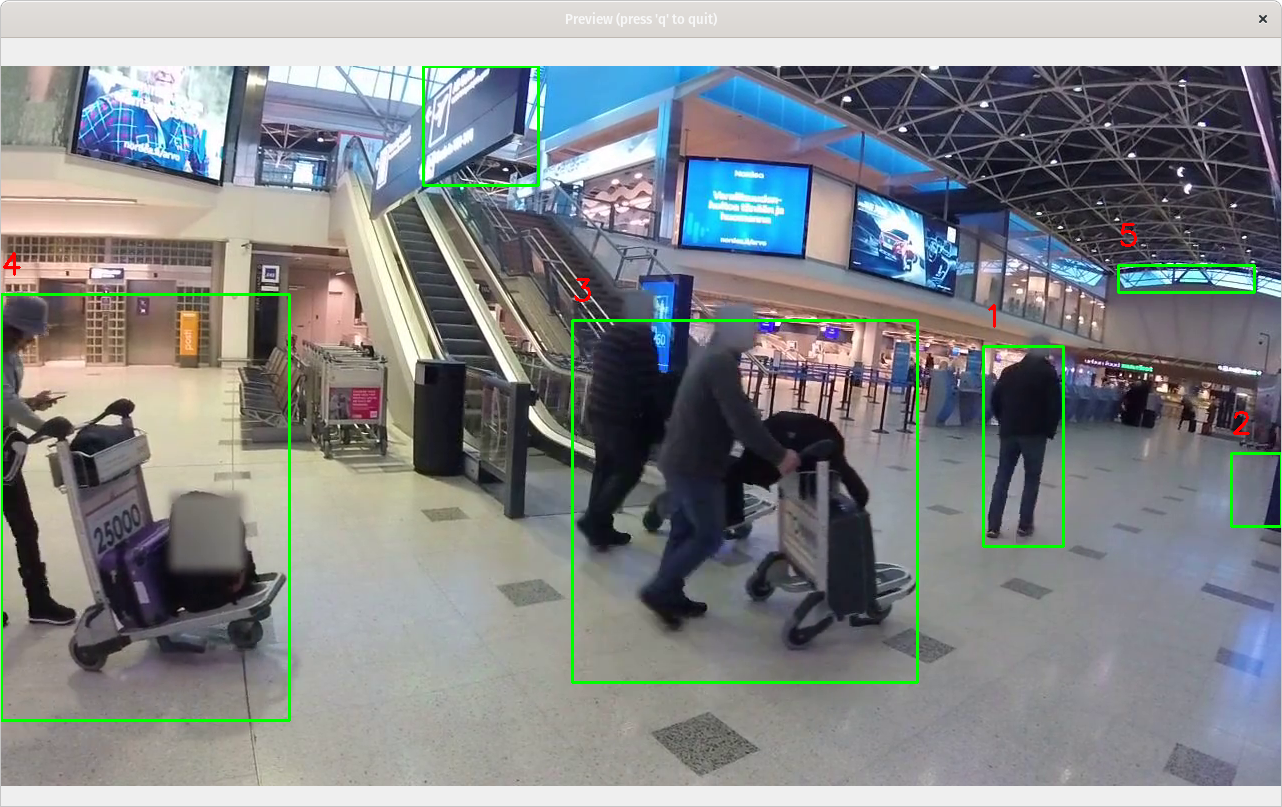
\includegraphics[scale=0.1]{figures/helsinki_bgsub}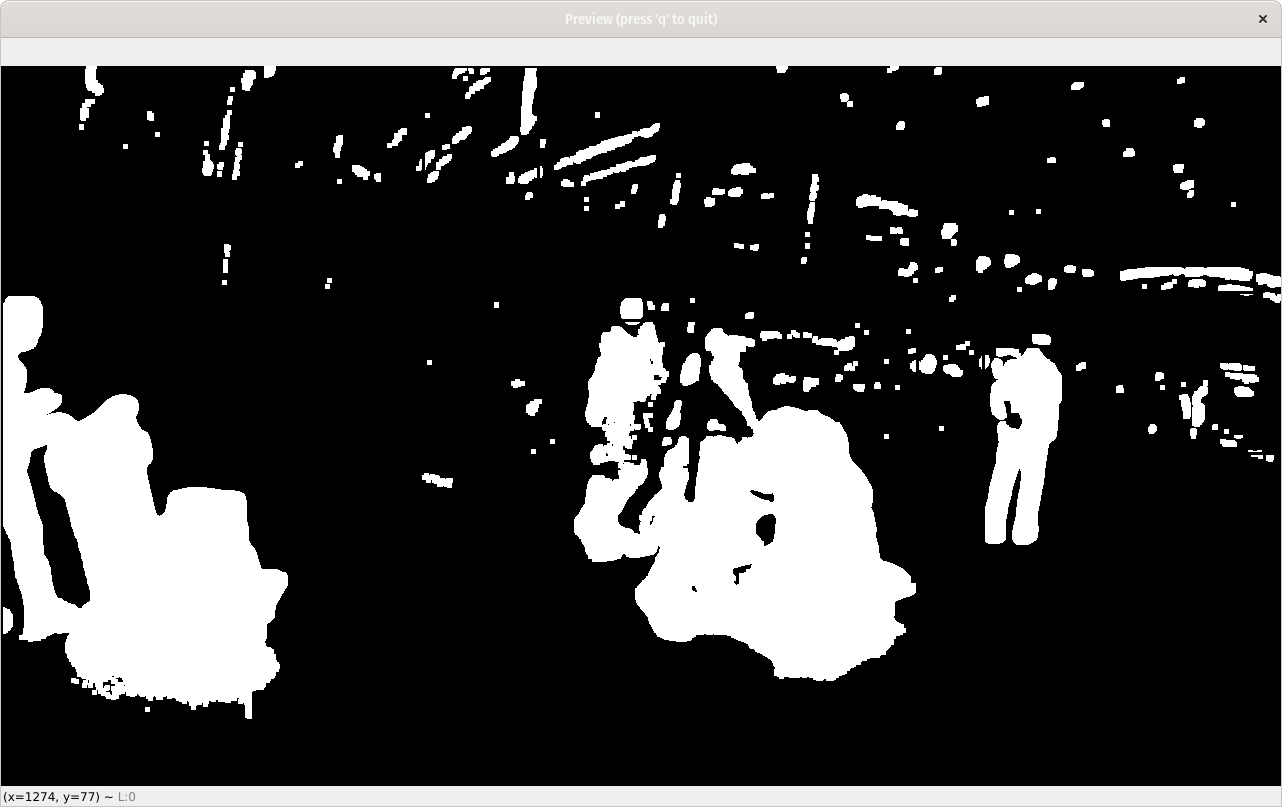
\includegraphics[scale=0.1]{figures/helsinki_bgsub_filtered}
\end{center}
\end{exampleblock}

\end{frame}

\begin{frame}{Dense Optical Flow}

\begin{itemize}
\item In addition to where motion is occurring, Dense Optical Flow estimates the \alert{direction and velocity} of motion relative to the 2D image.

\item Optical Flow is more computationally demanding, but can handle occluded objects with different trajectories.

\item Optical Flow can be computed efficiently through \alert{Farneb\"ack's method} \cite{farnemack}.\\[4mm]
\end{itemize}

\begin{exampleblock}{Example (TAU Urban A/V Scenes Dataset \cite{wang_curated_2021})}
\begin{center}
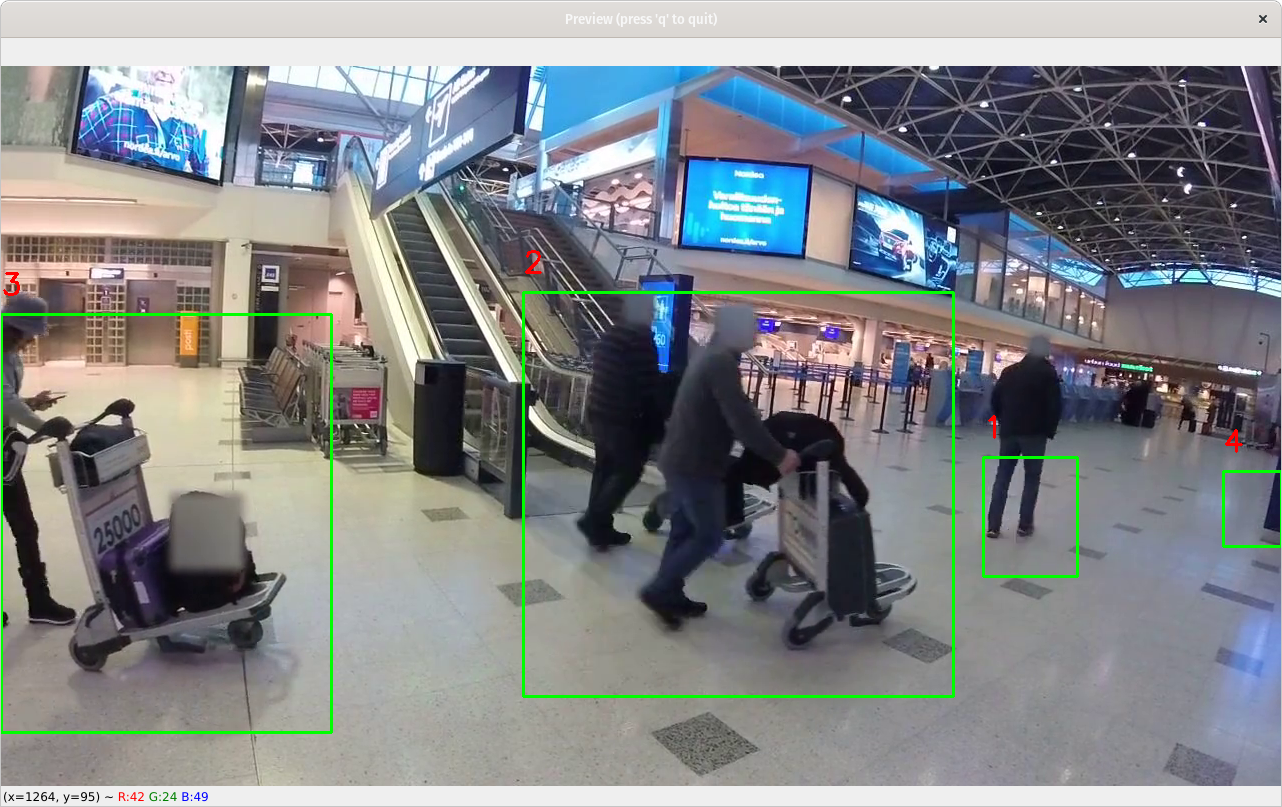
\includegraphics[scale=0.1]{figures/helsinki_optflow}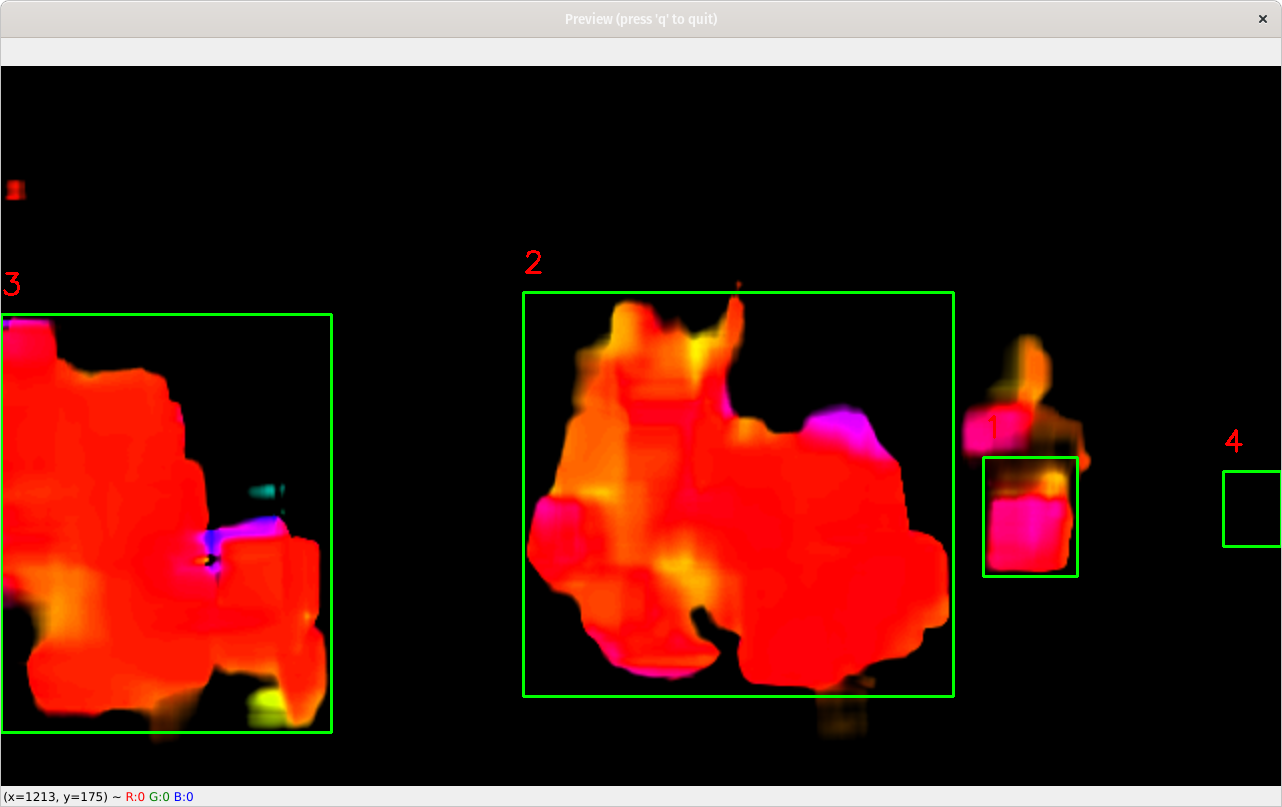
\includegraphics[scale=0.1]{figures/helsinki_optflow_filtered}
\end{center}
\end{exampleblock}

\end{frame}

\begin{frame}{TinyYOLO (CNN Object Detector)}

\begin{itemize}

\item The YOLO Model (``\textit{You Only Look Once}") is a Convolution Neural Network (CNN) that can identify and classify objects in a scene.

\item It is computationally demanding, but can be trained to identify only moving objects that are of interest in the scene.

\item The plugin prototype currently uses the pre-trained ``TinyYOLOv2" network, which has 9 layers, and over 15,000,000 trainable parameters.\\[4mm]

\end{itemize}

\begin{exampleblock}{Example (TAU Urban A/V Scenes Dataset \cite{wang_curated_2021})}
\begin{center}
\includegraphics[scale=0.1]{figures/helsinki_yolo}
\end{center}
\end{exampleblock}

\end{frame}

\section{Goals and Future Work}

\begin{frame}{Goals}
My Goals for this internship are the following:

\begin{enumerate}
\item I have little experience with computer vision, so I want to learn as much as possible about some of tools used in this field (OpenCV, etc.)

\item I'd like to produce a usable final product that will contribute to the Waggle project in a meaningful way.

\item I'd like to learn more about the mathematics of computer vision.

\item I want to meet some great people at Argonne and learn as much as I can from them.

\item I also want to be a great person to work with. 
\end{enumerate}
\end{frame}

\begin{frame}{Future Work}


My current priority list for my Waggle plugin project is the following:

\begin{enumerate}
\item Integrate the plugin prototype with PyWaggle so that it can publish object data to other plugins.

\item Begin work on more thorough documentation of the plugin.

\item Explore some ways of improving upon the aforementioned methods.

\item Allow for the plugin to import custom-trained object detection models.

\item Implement any suggestions and feedback from my mentors!
\end{enumerate}

\end{frame}

{\setbeamercolor{palette primary}{fg=White, bg=Meteorite}
\begin{frame}[standout]
  Questions?\\[10mm]
  \small{
  My Daily Progress Log:
  \href{https://github.com/waggle-sensor/summer2021/tree/main/Burdine}{https://github.com/waggle-sensor/summer2021/tree/main/Burdine}\\[6mm]
  Motion Detector Plugin:\\[2mm]
  \href{https://github.com/waggle-sensor/plugin-motion-detector}{https://github.com/waggle-sensor/plugin-motion-detector}}
\end{frame}
}

\begin{frame}[allowframebreaks]
\frametitle{References}
\bibliographystyle{amsalpha}
\bibliography{project_intro}
\end{frame}

\appendix

\section{Appendix}

\begin{frame}{YOLOv1 Architecture}
\begin{center}
\includegraphics[scale=0.3]{figures/yolo_cnn}\\
(This image is from the original YOLO paper \cite{YOLO})
\end{center}
\end{frame}

\end{document}
